%\VignetteIndexEntry{STK++ Arrays, User Guide}

\documentclass[a4paper,10pt]{article}

%-------------------------
% preamble for nice lsitings and notes

%-------------------
% Useful packages
\usepackage[utf8]{inputenc}
\usepackage[T1]{fontenc}

\usepackage{amsmath,amssymb,amsthm}
\usepackage[english]{babel}
\usepackage{graphicx}
\usepackage{geometry}
\usepackage{float}

\usepackage{url}
\usepackage{hyperref}
\usepackage{Sweave}

%-------------------
% Useful macros
\newcommand{\Rcpp}{{\tt Rcpp}} %
\newcommand{\rtkpp}{{\tt rtkpp}} %
\newcommand{\rtkore}{{\tt rtkore}} %
\newcommand{\stkpp}{{\tt STK++}} %
\newcommand{\Cpp}{{\tt C++}}

\newcommand{\Esp}[1]{\mathbb{E}\left[#1\right]}
\newcommand{\Var}[1]{\mathrm{Var}\left[#1\right]}
\newcommand{\E}[1]{\mathbb{E}\left[#1\right]}
\newcommand{\V}[1]{\mathrm{Var}\left[#1\right]}
\newcommand{\Loi}[1]{\mathcal{L}\left(#1\right)}

%----- Sets : integers, reals, complexes -----
\newcommand{\Nn}{\mathbb{N}} \newcommand{\N}{\mathbb{N}}
\newcommand{\Zz}{\mathbb{Z}} \newcommand{\Z}{\mathbb{Z}}
\newcommand{\Qq}{\mathbb{Q}} \newcommand{\Q}{\mathbb{Q}}
\newcommand{\Rr}{\mathbb{R}} \newcommand{\R}{\mathbb{R}}
\newcommand{\Cc}{\mathbb{C}}

%-------------------
% Multiple lines in a tabular
\newcommand{\vcell}[2][c]{%
\begin{tabular}[#1]{@{}l@{}}#2\end{tabular}}

%-------------------
% Nice notes and warnings
\usepackage{mdframed} % Add easy frames to paragraphs
\usepackage{xcolor}
\usepackage{xparse} % Add support for \NewDocumentEnvironment
\definecolor{graylight}{cmyk}{.30,0,0,.67} % define color using xcolor syntax
\definecolor{redlight}{rgb}{1,.2,.2}       % define color using xcolor syntax

\newmdenv[ % Define mdframe settings and store as leftrule
  linecolor=graylight,
  topline=false,
  bottomline=false,
  rightline=false,
  skipabove=\topsep,
  skipbelow=\topsep
]{leftrule}

\newmdenv[ % Define mdframe settings and store as leftrule
  linecolor=redlight,
  topline=false,
  bottomline=false,
  rightline=false,
  skipabove=\topsep,
  skipbelow=\topsep
]{redleftrule}

\NewDocumentEnvironment{note}{O{\textbf{Note:}}} % Define example environment
{\begin{leftrule}\noindent\textcolor{graylight}{#1}\par}
{\end{leftrule}}

\NewDocumentEnvironment{warning}{O{\textbf{Warning:}}} % Define warning environment
% environment
{\begin{redleftrule}\noindent\textcolor{redlight}{#1}\par}
{\end{redleftrule}}

%-------------------
% nice listing
\usepackage{listings}
\usepackage{caption}

\lstdefinestyle{customcpp}{
  language=C++,
  belowcaptionskip=1\baselineskip,
  breaklines=true,
  basicstyle=\ttfamily\scriptsize,
  frame=single,
  xleftmargin=\parindent,
  showstringspaces=false,
  keywordstyle=\color{red},
  commentstyle=\ttfamily\scriptsize\color{green!40!black},
  identifierstyle=\color{blue},
  stringstyle=\color{orange},
}
\lstdefinestyle{inlinecpp}{
  language=C++,
  belowcaptionskip=1\baselineskip,
  basicstyle=\ttfamily,
  frame=single,
  xleftmargin=\parindent,
  showstringspaces=false,
  keywordstyle=\color{red},
  commentstyle=\ttfamily\color{green!40!black},
  identifierstyle=\color{blue},
  stringstyle=\color{orange},
}


\DeclareCaptionFormat{listing}
{
  \colorbox[cmyk]{0.43, 0.35, 0.35, 0.01}
  { \parbox{\textwidth}{\hspace{15pt}#1#2#3}}
}
\captionsetup[lstlisting]{ format=listing, %labelfont=white, textfont=white
                         , singlelinecheck=false, margin=-0.2cm
                         , font={bf,footnotesize} }

\newcommand{\includelstlisting}[1]{\lstinputlisting[style=customcpp]{#1}}
\newcommand{\code}[1]{\lstinline[style=inlinecpp]@#1@}
\newcommand{\ttcode}[1]{{\ttfamily\scriptsize #1}}
% end nice listing
%---------------------



\geometry{top=3cm, bottom=3cm, left=2cm, right=2cm}

%% need no \usepackage{Sweave.sty}
% Title Page
\title{ User Guide: STK++ Arrays}
\author{Serge Iovleff}
\date{\today}

% start documentation
\begin{document}
\input{rtkpp-Arrays-concordance}

\maketitle
\begin{abstract}
This user guide gives a general review of the STK++ arrays and of their usages.
After giving a general review of the capability of the library, we detail the
various accessors/mutators available. We give a complete list of
constructors. We focus on the Array2D class and give some hints about their
capabilities. We then present the different visitors, appliers and functors
implemented in STK++ allowing to compute quantities or arrays of interests. We
then explain how it is possible to use or modify slices of arrays. Finally we end
this document by detailing the way to construct reference arrays.
\end{abstract}

\section{Introduction}

The containers/arrays you use in order to store and process the data in your
application greatly influence the speed and the memory usage of your application.
STK++ proposes a large choice of containers/arrays and methods that you can used
in conjunction with them.

There are mainly two kinds of arrays you can use with STK++:
\begin{itemize}
\item The \code{Array2D} family classes which are the classes defined in the
oldest versions of STK++,
\item the \code{CArray} family classes which have been introduced in version
0.4 of STK++ library.
\item For \rtkore{} users, the \code{RVector} and \code{RMatrix} wrap the
R \code{SEXP} stucture.
\end{itemize}

Before explaining the usage and differences between the different arrays,
we first introduce some vocabulary. The terminology used in STK++ project for
the arrays is the following:
\begin{itemize}
\item An array is often called a matrix.
\item In the case where a matrix has 1 column, such matrix is called
column-vector, often abbreviated just as \emph{vector},
\item in the other case, where a matrix has 1 row, it is called row-vector,
often abbreviated just as \emph{point}.
\end{itemize}

The word \emph{point} is borrowed from the statistical vocabulary where a row
of a data array is often named a point.

The \code{Array2D} classes are very flexible if you need to add, insert, remove,
resize,... quickly rows or columns to your container. On the other hand, the
storing scheme of the the CArray classes allow you to used them easily with
other linear algebra libraries (e.g. Lapack, Blas, ...).

\section{A detailed introductory example}
Consider the following example:

\begin{minipage}[t]{0.66\textwidth}
\lstinputlisting[style=customcpp,caption=Introductory example]{programs/tutoAccessors.cpp}
\end{minipage}
\hspace{0.2cm}
\begin{minipage}[t]{0.33\textwidth}
\addtocounter{lstlisting}{-1}
\lstinputlisting[style=customcpp,caption=Output]{programs/tutoAccessors.out}
\end{minipage}

\subsection{Accessors}
The primary coefficient accessors and mutators in STK++ are the overloaded
parenthesis operators. For matrices, the row index is always
passed first.

The \code{operator[]} is also overloaded for index-based access in
vectors, but keep in mind that \Cpp{} doesn't allow \code{operator[]} to take
more than one argument. The \code{operator[]} is thus restricted to
vectors/points/diagonal matrices. For vectors, just pass one index in a bracket.

Indexing starts at 0 by default. This behavior can be modify by defining the
STKBASEARRAYS macro at compile time using the directive -DSTKBASEARRAYS=1.
Enabling this macro allow user to get 1 based arrays like in FORTRAN.
If you want to build code independent of the start index you should use the
\code{beginCols()}, \code{beginRows()}, \code{endRows()}, \code{endCols()},
\code{lastIdxCols()} and \code{lastIdxRows()} methods of the arrays and the
\code{begin()}, \code{end()}, \code{lastIdx()} methods of the Row-vectors,
Column-Vectors, square matrices and diagonal matrices.

Here an example

\begin{minipage}[t]{0.66\textwidth}
\lstinputlisting[style=customcpp,caption=Accessors]{programs/tutoAccessors2.cpp}
\end{minipage}
\hspace{0.2cm}
\begin{minipage}[t]{0.33\textwidth}
\addtocounter{lstlisting}{-1}
\lstinputlisting[style=customcpp,caption=Output]{programs/tutoAccessors2.out}
\end{minipage}

\subsection{Expression template}

Assume that \code{c, a, d} are arrays of the same size and consider the line of
code
\begin{lstlisting}[style=customcpp]
c= -a - d  + 3.;
\end{lstlisting}
It is an expression involving matrix operations. All these expressions
are encoded in an expression template and are completely inlined at compile
time. It means there is no temporary objects created when these expressions
are evaluated.

\subsection{Constructors}

The \code{Array2D} family have only one mandatory template parameter: the type
of the data that will be stored. On the other hand arrays in \code{CArray}
family have four template parameters:
\begin{enumerate}
\item the type of the data that will be stored,
\item the number of rows (\code{UnknownSize} if it is not known at compile time),
\item the number of columns (\code{UnknownSize} if it is not known at compile time),
\item the orientation storage scheme of the data (by row or by column).
\end{enumerate}
Only the first template parameter is mandatory.

\begin{minipage}[t]{0.99\textwidth}
\lstinputlisting[style=customcpp,caption=Constructors]{programs/tutoConstructors.cpp}
\end{minipage}

\subsection{Accessing rows/columns/parts of an array}

You can access rows, columns and sub-part of STK++ arrays easily. Here is an example:

\begin{minipage}[t]{0.66\textwidth}
\lstinputlisting[style=customcpp,caption=Example]{programs/tutoSubArrays.cpp}
\end{minipage}
\hspace{0.2cm}
\begin{minipage}[t]{0.33\textwidth}
\addtocounter{lstlisting}{-1}
\lstinputlisting[style=customcpp,caption=Output]{programs/tutoSubArrays.out}
\end{minipage}

Applied to a vector/point/diagonal matrix the method sub require only
one parameter: the Range of the data we want to access/mutate.

In the general case, you can use the following methods in order to access/mutate
columns/rows/part of an array:
\begin{lstlisting}[style=customcpp,caption=Review of the main accessors]
// access to the ith row
 a.row(i);
// access to the element [first, first+size-1] of the ith row
 a.row(i, Range(first, size));
// access to the jth column
 a.col(j);
// access to the element [first, first+size-1] of the jth columns
 a.col(j, Range(first, size));
// access to the element [first, first+size-1] of the jth columns
 a.col(j, Range(first, size));
// Create ranges
 Range I(3,2), J(4,2);
// access to the sub-array formed by the range I,J.
 a.sub(I, J);
// access to the row i, in the range J = 4:5
 a(i,J);
 // access to the column j in the Range I=3:4
 a(I,j);
 // access to a subarray in the range (3:4, 4:5)
 a(I,J);
\end{lstlisting}


\subsection{Using references and move}

In some cases, you may want to conserve an access to some part of an array
for some work. For this purpose, it is possible to create reference
array, that is array that wrap (part of) another array

\begin{minipage}[t]{0.66\textwidth}
\lstinputlisting[style=customcpp,caption=reference
and move]{programs/tutoReferenceAndMove.cpp}
\end{minipage}
\hspace{0.2cm}
\begin{minipage}[t]{0.33\textwidth}
\addtocounter{lstlisting}{-1}
\lstinputlisting[style=customcpp,caption=Output]{programs/tutoReferenceAndMove.out}
\end{minipage}

The \code{Stat::mean} function return an \code{Array2D} \emph{by value}. In
order to avoid a useless copy, we use the \code{move} function. The following
piece of code
\begin{lstlisting}[style=customcpp]
a.move(b);
\end{lstlisting}
perform the operations:
\begin{itemize}
\item if \code{a} contains data, the memory is released,
\item \code{a} become the owner of the data contain by \code{b},
\item \code{b} become a reference,
\item If \code{b} was a reference, then \code{a}  is also a reference.
\end{itemize}

\begin{note}
Many more examples can be found in the test files coming with the STK++ library.
\end{note}

\section{Arrays classes and their constructors}

As say in the Introduction, there is two kind of arrays provides by the STK++ library: the
arrays part of the \code{Array2D} family and the arrays part of the \code{CArray} family.
Constructors depends of the structure of the array you want to obtain. In
this part we will review all the existing arrays and the different way
to create them.


\subsection{Review of the classes}

\subsubsection{\ttcode{Array2D} and \ttcode{CArray} classes}
The \code{Array2D} and \code{CArray} classes are the most general
classes for storing scalars. The values are stored in an array of range
\code{[beginRows:endRows)}$\times$\code{[beginCols:endCols)}.

\begin{lstlisting}[style=customcpp]
template<typename Type> class Array2D;
template< typename Type, int SizeRows_ = UnknownSize, int SizeCols_ = UnknownSize, bool Orient_ = Arrays::by_col_>
class CArray;
\end{lstlisting}

\subsubsection{\ttcode{Array2DVector}, \ttcode{Array2DPoint},  \ttcode{CArrayVector} and \ttcode{CArrayPoint} classes}

The \code{Array2DVector}, \code{Array2DPoint},  \code{CArrayVector}
and  \code{CArrayPoint} classes allow to store scalars in column and row
vectors. The values are stored in arrays of range \code{[begin:end)}.

\begin{lstlisting}[style=customcpp]
template<typename Type> Array2DVector;
template<typename Type> Array2DPoint;
template< typename Type, int SizeRows_=UnknownSize, bool Orient_ = Arrays::by_col_> class CArrayVector;
template< typename Type, int SizeCols_=UnknownSize, bool Orient_ = Arrays::by_row_> class CArrayPoint;
\end{lstlisting}

\begin{note}
Only the first template parameter is mandatory.
\end{note}

\subsubsection{\ttcode{Array2DSquare} and \ttcode{CArraySquare} classes}

The \code{Array2DSquare} and  \code{CArraySquare} classes are general classes for storing scalars in
a square matrix. The values are stored in an array of range \code{[begin:end)}$\times$\code{[begin:end)}.

\begin{lstlisting}[style=customcpp]
template<typename Type> Array2DSquare;
template< typename Type_, int Size_ = UnknownSize, bool Orient_ = Arrays::by_col_>
class CArraySquare;
\end{lstlisting}

\begin{note}
Only the first template parameter is mandatory.
\end{note}


\subsubsection{\ttcode{Array2DDiagonal} class}


The \code{Array2DDiagonal} class is a general class for storing scalars in
a diagonal matrix. The values are stored in an array of range
\code{[begin:end)}$\times$\code{[begin:end)} with zero outside the diagonal.


\begin{lstlisting}[style=customcpp]
template<typename Type> Array2DDiagonal;
\end{lstlisting}

\begin{note}
Only the diagonal values are effectively stored in an \code{Array2DDiagonal} array.
\end{note}

\subsubsection{\ttcode{Array2DUpperTriangular} and  \ttcode{Array2DLowerTriangular} classes}

The  \code{Array2DUpperTriangular} and  \code{Array2DLowerTriangular} classes are
general classes for storing scalars in triangular matrices.
The values are stored in an array of range
\code{[beginRows:endRows)}$\times$\code{[beginCols:endCols)} with zero in the
respectively lower and upper part of the array.


\begin{lstlisting}[style=customcpp]
template<typename Type> Array2DUpperTriangular;
template<typename Type> Array2DLowerTriangular;
\end{lstlisting}

\begin{note}
Only the non-zeros values are effectively stored in the arrays and
the upper part (respectively the lower part) is the part of the array such
that $j>i$ (resp. $i>j$), where $i$ represents the index of the row and $j$ the index
of the column.
\end{note}

\subsection{Constructors for the \ttcode{Array2D} family containers}

\subsubsection{Default constructors}
All default constructors create an empty Array of scalar \code{Type}
\begin{lstlisting}[style=customcpp]
Array2D<Type> a;
Array2DVector<Type> v;
Array2DPoint<Type> p;
Array2DSquare<Type> s;
Array2DDiagonal<Type> d;
Array2DLowerTriangular<Type> l;
Array2DUpperTriangular<Type> u;
\end{lstlisting}

In the following example
\begin{lstlisting}[style=customcpp]
Array2D<Real> a; // a is an empty array of Real (double by default)
a.resize(10,10)=0.; // a is now an array of size (10,10) with the value 0.
Array2DVector<Real> b; // a is an empty column vector of Real
b.resize(10)=0.; // b is now an column-vector of size 10 with the value 0.
\end{lstlisting}

\subsubsection{Constructors with given dimensions}
It is possible to declare an array with fixed ranges for the rows and the columns and
Optionally an initial value
\begin{lstlisting}[style=customcpp]
Array2D<Type>( Range const& I, Range const& J);
Array2D<Type>( Range const& I, Range const& J, Type const& v);
Array2DVector<Type>( Range const& I);
Array2DVector<Type>( Range const& I, Type const& v);
Array2DPoint<Type>( Range const& J);
Array2DPoint<Type>( Range const& J, Type const& v);
Array2DSquare<Type>( Range const& I);
Array2DSquare<Type>( Range const& I, Type const& v);
Array2DDiagonal<Type>( Range const& I);
Array2DDiagonal<Type>( Range const& I, Type const& v);
Array2DLowerTriangular<Type>( Range const& I, Range const& J);
Array2DLowerTriangular<Type>( Range const& I, Range const& J, Type const& v);
Array2DUpperTriangular<Type>( Range const& I, Range const& J);
Array2DUpperTriangular<Type>( Range const& I, Range const& J, Type const& v);
\end{lstlisting}

The following code build an array of \code{Real} (double by default) with rows in
the range $2:4$ and columns in the range $0:9$ (this is the default, but could be
$1:10$ if the macro STKBASEARRAYS=1 is activated). The array is initialized with
the value 2
\begin{lstlisting}[style=customcpp]
Array2D<Real> a(Range(2,3), 10, 2.);
\end{lstlisting}

The following code build a vector of \code{Real} (double by default) with columns
in the range $0:9$ (this is the default, but could be $1:10$ if the macro \ttcode{STKBASEARRAYS=1}
is activated). The array is initialized with the value $2$
\begin{lstlisting}[style=customcpp]
Array2DVector<Real> a( 10, 2.);
\end{lstlisting}

\subsubsection{Copy constructors}
All arrays have a copy constructor. In the following examples, the resulting array is either a
copy of the array \code{T} (if \code{ref == false}) or a reference of the array \code{T}  (if \code{ref == true})
\begin{lstlisting}[style=customcpp]
Array2D<Type>( Array2D<Type> const& T, bool ref=false) a; // a is a physical copy of T
Array2DVector<Type>( Array2DVector<Type> const& T, bool ref=false) v;  // v is a physical copy of T
Array2DPoint<Type>( Array2DPoint<Type> const& T, bool ref=false);
Array2DSquare<Type>( Array2DSquare<Type> const& T, bool ref=false);
Array2DDiagonal<Type>( Array2DDiagonal<Type> const& T, bool ref=false);
Array2DLowerTriangular<Type>( Array2DLowerTriangular<Type> const& T, bool ref=false);
Array2DUpperTriangular<Type>( Array2DUpperTriangular<Type> const& T, bool ref=false);
\end{lstlisting}

The following code copy the array \code{a} in a new array \code{b} and create a
reference of the rows and columns of \code{c} with range $I$ for the rows and
range $J$ for the columns.
\begin{lstlisting}[style=customcpp]
Array2D<Real> a(10, 8);
Array2D<Real> b(a); // b is now a copy of a
// c is a reference, if an element of c is modified, the corresponding element of a is modified
Array2D<Real> c(a.sub(I,J), true);
\end{lstlisting}

The following shows how to get a reference on a column and a reference on a row of an \code{Array2D}.
\begin{lstlisting}[style=customcpp]
Array2D<Real> a(10, 8);
Array2DVector<Real> c(a.col(1), true); // c is now a reference on the column 1 of a
Array2DPoint<Real> p(a.row(1), true); // p is now a reference on the row 1 of a
\end{lstlisting}

\begin{warning}
It is the responsibility of the user to verify that a reference is valid.
\end{warning}

\subsection{Constructors for the \ttcode{CArray} family containers}
\subsubsection{Default constructors}
All default constructors create an empty Array of scalar \code{Type}
\begin{lstlisting}[style=customcpp]
CArray<typename Type, SizeRows_, SizeCols_ = UnknownSize, bool Orient_ = Arrays::by_col_ >();
Array2DVector<typename Type, int Size_ = UnknownSize, bool Orient_ = Arrays::by_col_>();
CArrayPoint<typename Type, int Size_ = UnknownSize, bool Orient_ = Arrays::by_row_>();
CArraySquare<typename Type, int Size_ = UnknownSize, bool Orient_ = Arrays::by_col_>();
\end{lstlisting}
\begin{note}
The only mandatory template argument is \code{Type}.
\end{note}

Here after are some more examples
\begin{lstlisting}[style=customcpp]
CArray<Real> a; // a is an empty array of Real (double by default)
a.resize(10,10) =0.; // a is now an array of size (10,10) with the value 0.
CArrayVector<Real> b; // a is an empty column vector of Real
b.resize(10) =0.; // b is now a column-vector of size 10 with the value 0.
\end{lstlisting}

\subsubsection{Constructors with given dimensions}

It is possible to construct an array with fixed ranges for the rows and the columns and
optionally an initial value.
\begin{lstlisting}[style=customcpp]
CArray<Type>( Range const& I, Range const& J);
CArray<Type>( Range const& I, Range const& J, Type const& v);
CArrayVector<Type>( Range const& I);
CArrayVector<Type>( Range const& I, Type const& v);
CArrayPoint<Type>( Range const& J);
CArrayPoint<Type>( Range const& J, Type const& v);
CArraySquare<Type>( Range const& I);
CArraySquare<Type>( Range const& I, Type const& v);
\end{lstlisting}
If the dimension is known at compile time, you can use the template arguments
\begin{lstlisting}[style=customcpp]
CArray<Type, 10, 10> a; // uninitialized array of fixed size (10,10)
CArray<Type, 10, 10> a(0,0,1)); // array of fixed size (10,10) with initial value 1
\end{lstlisting}
The following code build an array of \code{Real} (double by default) with rows in
the range $2:4$ and columns in the range $0:9$ (this is the default, but could be
$1:10$ if the macro \ttcode{STKBASEARRAYS=1} is activated). The array is initialized with
the value $2$.
\begin{lstlisting}[style=customcpp]
CArray<Real> a(Range(2,3), 10, 2.);
\end{lstlisting}
The following code build a vector of \code{Real} (double by default) with columns
in the range $0:9$ (this is the default, but could be $1:10$ if the macro \ttcode{STKBASEARRAYS=1}
is activated). The array is initialized with the value $2$.
\begin{lstlisting}[style=customcpp]
CArrayVector<Real> a( 10, 2.);
\end{lstlisting}

\subsubsection{Copy constructors}

In the following examples, the resulting array is either a copy of the array \code{T} (if \code{ref == false})
or a reference of the array \code{T}  (if \code{ref == true})
\begin{lstlisting}[style=customcpp]
CArray<Type>( const CArray<Type> const& T, bool ref=false);
CArrayVector<Type>( CArrayVector<Type> const& T, bool ref=false);
CArrayPoint<Type>( CArrayPoint<Type> const& T, bool ref=false);
CArraySquare<Type>( CArraySquare<Type> const& T, bool ref=false);
\end{lstlisting}

The following code copy the array \code{a} in a new array \code{b} and create a
reference of the rows and columns of \code{c} with range $I$ for the rows and
range $J$ for the columns
\begin{lstlisting}[style=customcpp]
CArray<Real> a(10, 8);
CArray<Real> b(a); // b is now a copy of a
// c is a reference, if an element of c is modified, the corresponding element of a is modified
CArray<Real> c(a.sub(I,J), true);
\end{lstlisting}
The following show how to get a reference on a column and a reference on a row of a \code{CArray}.
\begin{lstlisting}[style=customcpp]
CArray<Real> a(10, 8);
CArrayVector<Real> c(a.col(1), true); // c is now a reference on the column 1 of a
CArrayPoint<Real> p(a.row(1), true); // p is now a reference on the row 1 of a
\end{lstlisting}

\section{Using \ttcode{Array2D} arrays}

This section explains how you can add and/or remove columns/rows to an array of
the \code{Array2D} family and how to merge arrays with the same number of rows
without duplicating data.

\subsection{General features of the \ttcode{Array2D}}

The \code{Array2D} is a family of array/vectors/points proposing much
functionality allowing to add/remove rows/columns. It is also possible to
resize them in a conservative way. It is also possible to merge them if the
dimensions agreed.

Each columns in an \code{Array2D} is in a contiguous memory block. Thus, all
operations on the columns are fast as it does not involve data copy. This is not
the case for the rows. Inserting or appending rows will cause in the worse cases,
that is if the number of rows required is greater than the capacities of the columns,
a re-allocation of a part (all) the columns.

\subsection{Adding rows and columns to \ttcode{Array2D}}

All the \code{Array2D} (That is the arrays deriving from the interface
class \code{IArray2D}) can add, insert, remove rows or columns to an existing
data set.

In this first example, we add columns to an \code{Array2D}

\begin{minipage}[t]{0.5\textwidth}
\lstinputlisting[style=customcpp,caption=Adding columns]{programs/tutoAddingCols.cpp}
\end{minipage}
\hspace{0.2cm}
\begin{minipage}[t]{0.5\textwidth}
\addtocounter{lstlisting}{-1}
\lstinputlisting[style=customcpp,caption=Output]{programs/tutoAddingCols.out}
\end{minipage}
And in this second example, we add rows to an \code{Array2D}

\begin{minipage}[t]{0.5\textwidth}
\lstinputlisting[style=customcpp,caption=Adding rows]{programs/tutoAddingRows.cpp}
\end{minipage}
\hspace{0.2cm}
\begin{minipage}[t]{0.5\textwidth}
\addtocounter{lstlisting}{-1}
\lstinputlisting[style=customcpp,caption=Output]{programs/tutoAddingRows.out}
\end{minipage}

\begin{note}
It is important to observe that adding/inserting columns to an \code{Array2D}
does not produce any copy of the data stored, while the same operations
involving the rows of the array will produce data movement.

The next graphic give the execution time of the following code
\begin{lstlisting}[style=customcpp]
   A.pushFrontCols(Const::VectorX(m));
   A.insertCols(2, 2);
   A.col(2) = A.col(1).square();
   A.col(3) = A.col(1).cube();
   A.pushBackCols(2);
   A.col(5) = A.col(4).square();
   A.col(6) = A.col(4).cube();
\end{lstlisting}
and of the same code by replacing "Cols" by "Rows". The size of the array
\code{A} was $(m,m)$. It is easily observed that adding rows is time consuming.
Observe also that a small amount of space is added at the creation of the
object and that the usage of the \code{reserve} method can be wise in order to
save time.

\begin{center}
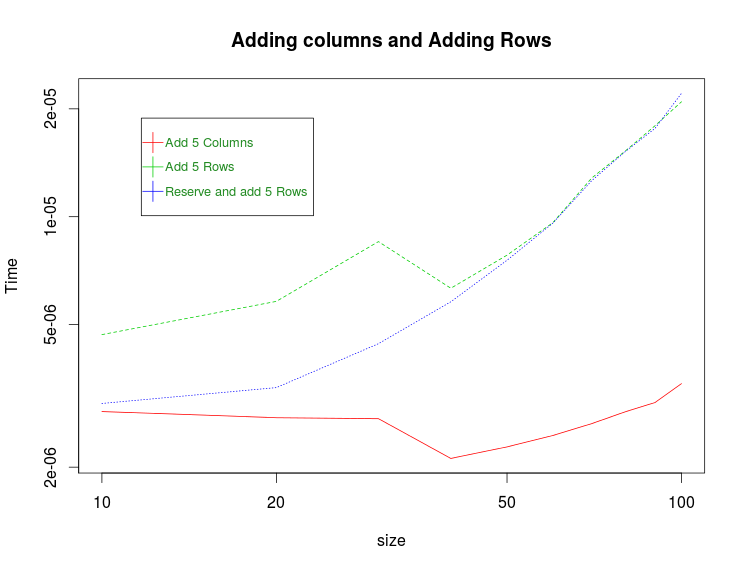
\includegraphics{images/benchAdd.png}
\end{center}
\end{note}

\subsection{Removing Rows and Columns}

Rows and columns can be also removed from arrays of the \code{Array2D} family
using \code{remove} and \code{popBack} methods.

\begin{minipage}[t]{0.5\textwidth}
\lstinputlisting[style=customcpp,caption=Removing rows and columns]{programs/tutoRemoveRowsAndCols.cpp}
\end{minipage}
\hspace{0.2cm}
\begin{minipage}[t]{0.5\textwidth}
\addtocounter{lstlisting}{-1}
\lstinputlisting[style=customcpp,caption=Output]{programs/tutoRemoveRowsAndCols.out}
\end{minipage}

\subsection{Merging two arrays}

It is possible to merge an array with an other array or vector without
copying the data using the merge method.

\begin{minipage}[t]{0.66\textwidth}
\lstinputlisting[style=customcpp,caption=Merge an array with an array and a vector]{programs/tutoMergeArrays2D.cpp}
\end{minipage}
\hspace{0.2cm}
\begin{minipage}[t]{0.33\textwidth}
\addtocounter{lstlisting}{-1}
\lstinputlisting[style=customcpp,caption=Output]{programs/tutoMergeArrays2D.out}
\end{minipage}

\section{Using Visitors, Appliers and Functors}

This page explains STK++'s visitors and appliers and how they
can be used on the arrays and in expressions.

\subsection{Visitors}

A visitor is a constant function applied to an expression or array
returning a single value. One of the most useful visitor is \code{ExprBase::sum()},
returning the sum of all the coefficients of a given expression or array.

Visitors can also be used to obtain the location of an element
inside an Expression or Array. This is the case of \code{ExprBase::maxElt(i,j)},
\code{ExprBase::maxElt(i) }, \code{ExprBase::minElt(i,j)} and \code{ExprBase::minElt(i)},
which can be used to find the location of the greatest or smallest coefficient in
an Expression or an Array.

The \code{minElt} method should not be confounded with the \code{min} method which compute
the minimum between two arrays.

The next example shows different usage of visitors

\begin{minipage}[t]{0.66\textwidth}
\lstinputlisting[style=customcpp,caption=Usage of the visitors]{programs/tutoVisitors.cpp}
\end{minipage}
\hspace{0.2cm}
\begin{minipage}[t]{0.33\textwidth}
\addtocounter{lstlisting}{-1}
\lstinputlisting[style=customcpp,caption=Output]{programs/tutoVisitors.out}
\end{minipage}

\subsection{Slicing Visitors}

A visitor can also be applied on each column/row of an Expression
or Array by using global functions in the \code{STK} namespace. All the visitors
can be used as slicing visitors except the \code{minElt} with arguments.

\begin{minipage}[t]{0.6\textwidth}
\lstinputlisting[style=customcpp,caption=Slicing visitors]{programs/tutoSlicingVisitors.cpp}
\end{minipage}
\hspace{0.2cm}
\begin{minipage}[t]{0.39\textwidth}
\addtocounter{lstlisting}{-1}
\lstinputlisting[style=customcpp,caption=Output]{programs/tutoSlicingVisitors.out}
\end{minipage}

\subsection{Appliers}

An applier is like a visitor except that it can only be applied to arrays
as it will modify the content of the array. Slicing appliers does not have
any meaning and thus an applier can only be used on a whole expression. If
you need to use an applier on a row or column use the \code{col} or \code{row} method.

\begin{minipage}[t]{0.5\textwidth}
\lstinputlisting[style=customcpp,caption=Appliers]{programs/tutoAppliers.cpp}
\end{minipage}
\hspace{0.2cm}
\begin{minipage}[t]{0.5\textwidth}
\addtocounter{lstlisting}{-1}
\lstinputlisting[style=customcpp,caption=Output]{programs/tutoAppliers.out}
\end{minipage}


\subsection{Functors}

Functors can fundamentally be used in the same way that slicing visitors. The
only difference is that they return an \code{Array2DPoint} if they are applied
by column or an \code{Array2DVector} if they are applied by rows. Recall that it
is possible to use the \code{move} method in order to store the results of the
computation without data copy.

All the functors computing statistics are in the \code{Stat} namespace and
compute the usual statistics by columns or rows. If there is the possibility
of missing/NaN values add the word \code{Safe} to the name of the functor. If
the mean by row is needed, just add ByRow to the name of the functor. If you
want both add SafeByRow.

\begin{minipage}[t]{0.5\textwidth}
\lstinputlisting[style=customcpp,caption=Functors]{programs/tutoStatFunctors.cpp}
\end{minipage}
\hspace{0.2cm}
\begin{minipage}[t]{0.5\textwidth}
\addtocounter{lstlisting}{-1}
\lstinputlisting[style=customcpp,caption=Output]{programs/tutoStatFunctors.out}
\end{minipage}




\section{Slicing arrays and expressions}

This part explains the slicing operations. A slice is a rectangular part of an
array or expression. Arrays slices can be used both as \ttcode{rvalue} and as \ttcode{lvalue}
while Expression slice can only be used as \ttcode{rvalue}.

\subsection{Rows and Columns}

Individual columns and rows of arrays and expressions can be accessed using
\code{ExprBase::col()} and \code{ExprBase::row()} as \ttcode{rvalue}
and using \code{ArrayBase::col()} and \code{ArrayBase::row()} methods as
\ttcode{lvalue}. The argument for \code{col()} and \code{row()} is the index
of the column or row to be accessed.

\begin{minipage}[t]{0.5\textwidth}
\lstinputlisting[style=customcpp,caption=Rows and columns slice]{programs/tutoRowsAndCols.cpp}
\end{minipage}
\hspace{0.2cm}
\begin{minipage}[t]{0.5\textwidth}
\addtocounter{lstlisting}{-1}
\lstinputlisting[style=customcpp,caption=Output]{programs/tutoRowsAndCols.out}
\end{minipage}


\subsection{sub-Arrays and sub-Vectors}

The most general sub operation  is named \code{sub()}. There are two versions, one
for arrays, an other for vectors. The sub-Arrays and sub-vectors can be
employed as \ttcode{rvalue} or \ttcode{lvalue}, meaning you can assign or reference a
sub-array or sub-vector.

\begin{minipage}[t]{0.5\textwidth}
\lstinputlisting[style=customcpp,caption=sub arrays and vectors]{programs/tutoSubArrays.cpp}
\end{minipage}
\hspace{0.2cm}
\begin{minipage}[t]{0.5\textwidth}
\addtocounter{lstlisting}{-1}
\lstinputlisting[style=customcpp,caption=Output]{programs/tutoSubArrays.out}
\end{minipage}

\section{Using reference arrays}

This part explains how to create reference on existing arrays.

\subsection{Creating reference to sub-arrays}

Any slice of an existing array can be referenced by an other array
and modified using this "reference" container. This is achieved
using the copy constructor with reference as \code{true}.

\begin{minipage}[t]{0.5\textwidth}
\lstinputlisting[style=customcpp,caption=Referencing sub-arrays]{programs/tutoReference.cpp}
\end{minipage}
\hspace{0.2cm}
\begin{minipage}[t]{0.5\textwidth}
\addtocounter{lstlisting}{-1}
\lstinputlisting[style=customcpp,caption=Output]{programs/tutoReference.out}
\end{minipage}

This method allows to get a safe access to some sub-part of a big array that
you want to modify.

\begin{warning}
It is the responsibility of the user to verify that a reference is valid.
\end{warning}

\subsection{Creating reference to raw data}

It is possible to map a single pointer \code{Type*} or a double pointer \code{Type**}
in respectively \code{CArray} and \code{Array2D} using the dedicated constructors.


In this constructor, we wrap the data pointed by \code{q} in an array with rows in
the range $I$ and columns in the range $J$.
\begin{lstlisting}[style=customcpp,caption=Wrapping raw data in Array2D]
Array2D<Type>( Type** q, Range const& I, Range const& J);
\end{lstlisting}

In this example we create an array of size (10,5) and wrap it in an \code{Array2D}.
\begin{lstlisting}[style=customcpp,caption=Example of wrapping by Array2D]
Real** q = new Real*[10];
for (int j=0; j<10; j++) { q[j] = new Real[5];}
//wrap q. Note that q will not be freed when a is deleted
Array2D<Real> a(q, Range(0,10), Range(0,5));
\end{lstlisting}


In this constructor, we wrap the data pointed by \code{q} in an array with rows
and columns of size $m$ and $n$.
\begin{lstlisting}[style=customcpp,caption=Wrapping raw data in CArray]
CArray<Type>( Type* q, int m, int n);
\end{lstlisting}

In this example we create an array of size (10, 5) and wrap it in a \code{CArray}.
\begin{lstlisting}[style=customcpp],caption=Example of wrapping by CArray]
Real* q = new Real[10];
for (int j=0; j<10; j++) { q[j] = j;}
//wrap q in a fixed size array of size (2,5).
// Note that q will not be freed when a is deleted
CArray<Real, 2, 5> a(q, 2, 5);
\end{lstlisting}


%\bibliographystyle{plain}
%\bibliography{rtkore}
\end{document}

